%%%%%%%%%%%%%%%%%%%%%%%%%%%%%%%%%%%%%%%%%%

\chapter{LANL nEDM experiment control and data acquisition systems}\label{chap:daq}

%%%%%%%%%%%%%%%%%%%%%%%%%%%%%%%%%%%%%%%%%%

This chapter primarily serves as documentation regarding the experimental control system and data acquisition (\acrshort*{daq}) system for the LANL nEDM experiment. We first describe the devices associated with $\pi/2$ pulse generation in the Ramsey method (Secs.~\ref{sec:pulse_gen_freq_std}). We then describe the system responsible for recording the pulse height spectra and timing of UCN detection events (Sec.~\ref{sec:fast_daq}). Lastly, we describe the current iteration of the experimental control system (Sec.~\ref{sec:slow_control}) and the envisioned final version (Sec.~\ref{sec:web_control}).

The majority of the code implemented this chapter is extremely lengthy. In lieu of an appendix, we provide links to the repositories hosted on GitHub in the table below.

\begin{table}[htp]
\renewcommand*{\arraystretch}{2}
\centering
\caption{Links to code repositories}\label{tb:github}
\begin{tabular}{
    l
    r
}
\toprule
Description & \href{https://github.com/dougUCN/}{github.com/dougUCN} \\
\midrule
SIS3316 Digitizer  & \href{https://github.com/dougUCN/SIS3316}{/SIS3316} \\
\makecell[l]{GPIB device communication\\(DS345, DG535, BNC577)} & \href{https://github.com/dougUCN/gpibUSB}{/gpibUSB} \\
Cell valve motor control & \href{https://github.com/dougUCN/STM23Q}{/STM23Q} \\
Switcher motor control &  \\
\makecell[l]{LANL nEDM Dec. 2023\\experimental control} & \\
ZeroMQ Communication & \href{https://github.com/dougUCN/zmqLANL}{/zmqLANL} \\
SIS3316 GUI & \\
Web-based control system (FE) & \href{https://github.com/dougUCN/LANE-client}{/LANE-client} \\
Web-based control system (BE) & \href{https://github.com/dougUCN/LANE-server}{/LANE-server} \\
\bottomrule
\end{tabular}
\end{table}


%%%%%%%%%%%%%%%%%%%%%%%%%%%%%%%%%%%%%%%%%%

\section{RF signal generators and frequency standard}\label{sec:pulse_gen_freq_std}

%%%%%%%%%%%%%%%%%%%%%%%%%%%%%%%%%%%%%%%%%%

The frequency generators for the $\pi/2$ RF coils and other timing systems in the experiment must have smaller uncertainty than the counting statistics from a single measurement cycle. From Sec.~\ref{sec:lanl_nedm_uncertainty}, the nEDM uncertainty per Ramsey sequence measurement for two cells is on the order of $\sim 10^{-25}\,e\text{ cm}$. From Eq.~(\ref{eq:delta_omega_dipole_relation}), for $E=\qty{12}{kV\per cm}$ this gives a frequency uncertainty of $\sigma(f)\sim \qty{1}{\micro Hz}$.

We use SRS DS345 signal generators to drive the $\pi/2$ RF coils. The accuracy is stated to be \qty{5}{ppm}~\cite{ds345_manual}, which for the $\approx\qty{30}{Hz}$ resonance in the LANL nEDM Ramsey sequence (Sec.~\ref{sec:LANL_nEDM_ramsey_params}) corresponds to $\qty{0.15}{mHz}$. This can be improved to at least $\qty{0.1}{\micro Hz}$ per measurement with synchronization to a SRS FS725 rubidium frequency standard, which we have procured. The FS725 has short-term \qty{1}{s} stability (Allan variance) and accuracy to a few parts in $10^{11}$, and long-term \qty{20}{yr} accuracy of \num{5e-9}~\cite{rubidium_standard_fs725_manual}.

A frequency uncertainty specification of $\sim \qty{1}{\micro Hz}$ gives a phase shift uncertainty per Ramsey measurement of $\sigma(\phi)=2\pi\gls{T_fp}\,\sigma(f)\sim \qty{1}{mrad}$. We performed a phase stability test, where a $V_\text{S}=\qty{1}{V}$, $f_\text{S}=\qty{30}{Hz}$ signal from a DS345 was input into a Signal Recovery 7265 lock-in amplifier. A second $V_\text{R}=\qty{1}{V}$, $f_\text{R}=\qty{30}{Hz}$ signal from another DS345, referenced to the FS725, was the reference. The lock in time constant was \qty{200}{ms}. The output phase was $\Phi=2\pi \Delta f\,t-\Delta\phi(t)$ where $\Delta f=f_\text{R}-f_\text{S}$ and $\Delta\phi(t)$ is the phase drift of the signal DS345 relative to the FS725 standard. The output phase increased at a rate of $d\Phi/dt=\qty{1.16e-4}{rad\per s}$, which assuming $\Delta f$ is the dominant contribution implies $\Delta f=\qty{18}{\micro Hz}$ (a true frequency of $f_\text{S}=\qty{29.999982}{Hz}$) and an accuracy of $\qty{18}{\micro Hz}/\qty{30}{Hz}=\qty{0.6}{ppm}$. Setting the input signal frequency to $\qty{30.000018}{Hz}$ resulted in $d\Phi/dt=\qty{5.82}{\micro rad\per s}$, which sets a bound $d\phi(t)/dt<\qty{5.82}{\micro Hz\per s}$. Over the a $\gls*{T_fp}=\qty{180}{s}$ free precession this gives a maximum shift of $\qty{1.05}{mrad}$, matching the phase uncertainty specification for a DS345 that is unsynchronized to the FS725. We anticipate that the DS345 phase drift when synchronized to the time standard is significantly smaller.

%%%%%%%%%%%%%%%%%%%%%%%%%%%%%%%%%%%%%%%%%%

\subsection{RF pulse and free precession timing}\label{sec:pulse_gates}

%%%%%%%%%%%%%%%%%%%%%%%%%%%%%%%%%%%%%%%%%%

Timing of the $\pi/2$ pulses and free precession period has previously been controlled with a DG535 pulse generator. As exemplified by the sequencing in Appx.~\ref{appx:gpib_usb_pulse_sequence}, the DG535 was used to adjust the output amplitude of the DS345 function generator. The DG535 has a delay resolution of \qty{5}{ps}, and a nominal channel-to-channel jitter of \qty{50}{ps}~\cite{dg535_manual}. An 8-channel BNC 577 pulse generator has also been procured in anticipation of other instrumentation that require precision timing, with a delay resolution of \qty{250}{ps} and channel-to-channel jitter of \qty{50}{ps}~\cite{bnc_577_manual}. Both pulse generators may be synchronized to the FS725 time standard, which would further improve their performance.

%%%%%%%%%%%%%%%%%%%%%%%%%%%%%%%%%%%%%%%%%%

\section{Data acquisition}\label{sec:fast_daq}

%%%%%%%%%%%%%%%%%%%%%%%%%%%%%%%%%%%%%%%%%%

The system responsible for recording the pulse height spectra and timing of UCN detection events is referred to as the ``fast DAQ.'' It has been rigorously tested, having been utilized in all nEDM commissioning measurements involving UCN detection since 2020. The signal conditioning chain after the detector is relatively minimal, and is described in Sec.~\ref{sec:signal_conditioning}. The LANL nEDM uses a \qty{250}{MHz} SIS3316 by Struck Innovative Systeme to digitize the conditioned output. A RESTful interface was originally written by Sergey Ryzhikov for the PANDA experiment at the Institute for High Energy Physics, but it was written in Python2 and had lost compatibility with any SIS3316 with firmware later than 2015. An updated version in Python3, compatible with all firmware released to date and with an expanded feature set, is at [\url{https://github.com/dougUCN/SIS3316}]. 

The manuals for the SIS3316~\cite{sis3316_manual, sis3316_udp_addendum} (available on the GitHub repository) provide ample documentation, but we highlight relevant specifications, triggering algorithms, and device communication protocols in Sec.~\ref{sec:sis3316_specs}--\ref{sec:sis3316_pileup}.

%%%%%%%%%%%%%%%%%%%%%%%%%%%%%%%%%%%%%%%%%%

\subsection{UCN detection signal conditioning}\label{sec:signal_conditioning}

%%%%%%%%%%%%%%%%%%%%%%%%%%%%%%%%%%%%%%%%%%

 \begin{figure}
    \centering
    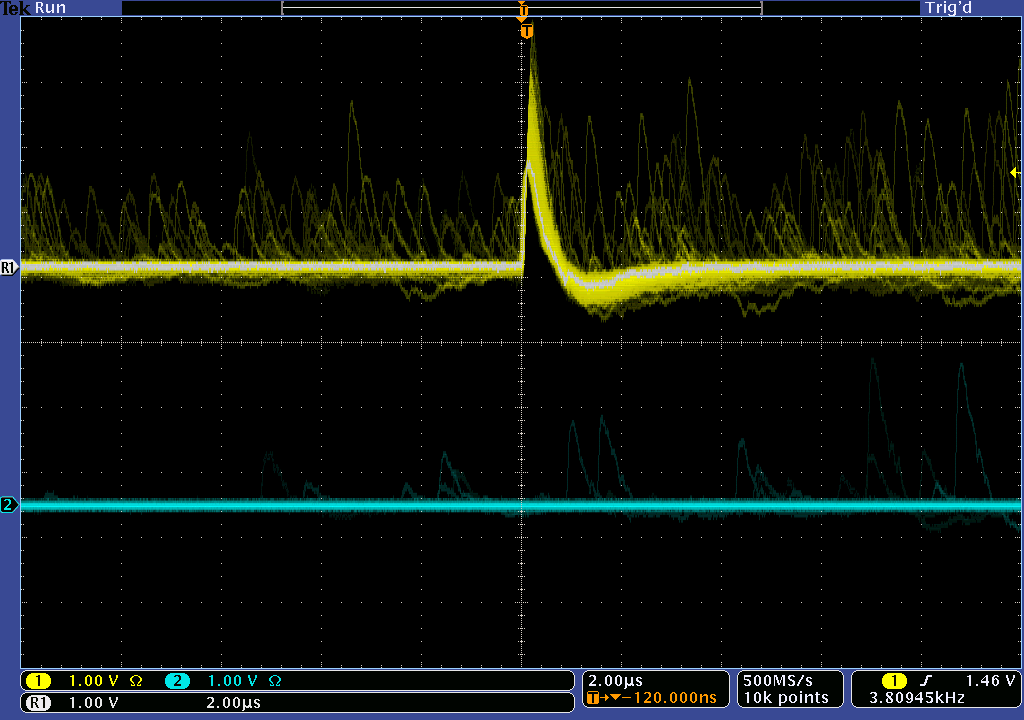
\includegraphics[width=0.8\textwidth]{figures/pmt_scope.png}
    \caption
     {UCN signals as viewed on an oscilloscope, after the PMT output is processed by an Ortec 474 timing filter amplifier}
    \label{fig:scope_image}
\end{figure}

After UCN are detected as per Sec.~\ref{sec:ucn_detectors}, the signal output from a \gls*{pmt} is to sent to an Ortec 474 timing filter amplifier. The integration time is set to \qty{500}{\nano\second}. Gain is set such that the pulse spectrum heights, when viewed on an oscilloscope, have an amplitude $\sim\qty{1}{\volt}$. The differentiation is nominally in the range of 0--\qty{20}{\nano\second}, set such that the pulse decays within \qty{5}{\micro \second}. An example UCN pulse shape is shown in Fig.~\ref{fig:scope_image}.

Initial tests of UCN with Onsemi \acrshort*{sipm} 4-Side Scaleable Arrays (C Series), used on the simultaneous spin analyzers, have shown that the output does not require the same pulse shaping as the PMTs. A custom fast-amplifier is being designed and built.

%%%%%%%%%%%%%%%%%%%%%%%%%%%%%%%%%%%%%%%%%%

\subsection{Struck SIS3316 specifications}\label{sec:sis3316_specs}

%%%%%%%%%%%%%%%%%%%%%%%%%%%%%%%%%%%%%%%%%%

Dead time calc

\cite{sis3316_manual, sis3316_udp_addendum}



%%%%%%%%%%%%%%%%%%%%%%%%%%%%%%%%%%%%%%%%%%

\subsection{Raw data format}

%%%%%%%%%%%%%%%%%%%%%%%%%%%%%%%%%%%%%%%%%%

%%%%%%%%%%%%%%%%%%%%%%%%%%%%%%%%%%%%%%%%%%

\subsection{Communication with the sis3316}\label{sec:sis3316_udp_protocol}

%%%%%%%%%%%%%%%%%%%%%%%%%%%%%%%%%%%%%%%%%%

UDP Protocol

Read/ack format

In order to maximize the data transfer rate, reduce the number of packets sent, and reduce the chances of a packet being dropped, we direct the sis3316 to use Jumbo frames, with a maximum transmission unit (MTU) of 9000 bytes. See Appx.~\ref{appx:sis3316_setup} for configuration of the sis3316 ethernet connection.

%%%%%%%%%%%%%%%%%%%%%%%%%%%%%%%%%%%%%%%%%%

\subsection{Trapezoid trigger algorithm}

%%%%%%%%%%%%%%%%%%%%%%%%%%%%%%%%%%%%%%%%%%

%%%%%%%%%%%%%%%%%%%%%%%%%%%%%%%%%%%%%%%%%%

\subsection{Pileup flagging}\label{sec:sis3316_pileup}

%%%%%%%%%%%%%%%%%%%%%%%%%%%%%%%%%%%%%%%%%%

%%%%%%%%%%%%%%%%%%%%%%%%%%%%%%%%%%%%%%%%%%

\section{Experiment control}\label{sec:slow_control}

%%%%%%%%%%%%%%%%%%%%%%%%%%%%%%%%%%%%%%%%%%

A LabJack-U3-LV and a PS12DC Power Switching Board attachment are used to communicate with the proton accelerator, beamline gate vales, and other systems that require a transistor-transistor logic (TTL) pulse for control.


%%%%%%%%%%%%%%%%%%%%%%%%%%%%%%%%%%%%%%%%%%

\subsection{Switchers}\label{sec:switcher_control}

%%%%%%%%%%%%%%%%%%%%%%%%%%%%%%%%%%%%%%%%%%



%%%%%%%%%%%%%%%%%%%%%%%%%%%%%%%%%%%%%%%%%%

\subsection{Cell valves}\label{sec:cell_valve_control}

%%%%%%%%%%%%%%%%%%%%%%%%%%%%%%%%%%%%%%%%%%


%%%%%%%%%%%%%%%%%%%%%%%%%%%%%%%%%%%%%%%%%%

\subsection{ZeroMQ device network}

%%%%%%%%%%%%%%%%%%%%%%%%%%%%%%%%%%%%%%%%%%

%%%%%%%%%%%%%%%%%%%%%%%%%%%%%%%%%%%%%%%%%%

\subsection{SIS3316 local GUI}

%%%%%%%%%%%%%%%%%%%%%%%%%%%%%%%%%%%%%%%%%%

Setup git repository. UI build in QT Designer, converted to python. Signals then connected in the main python... (mimic stuff that should go in the readme)

%%%%%%%%%%%%%%%%%%%%%%%%%%%%%%%%%%%%%%%%%%

\section{Web-based control system: proof of concept}\label{sec:web_control}

%%%%%%%%%%%%%%%%%%%%%%%%%%%%%%%%%%%%%%%%%%


\begin{figure}
    \centering
    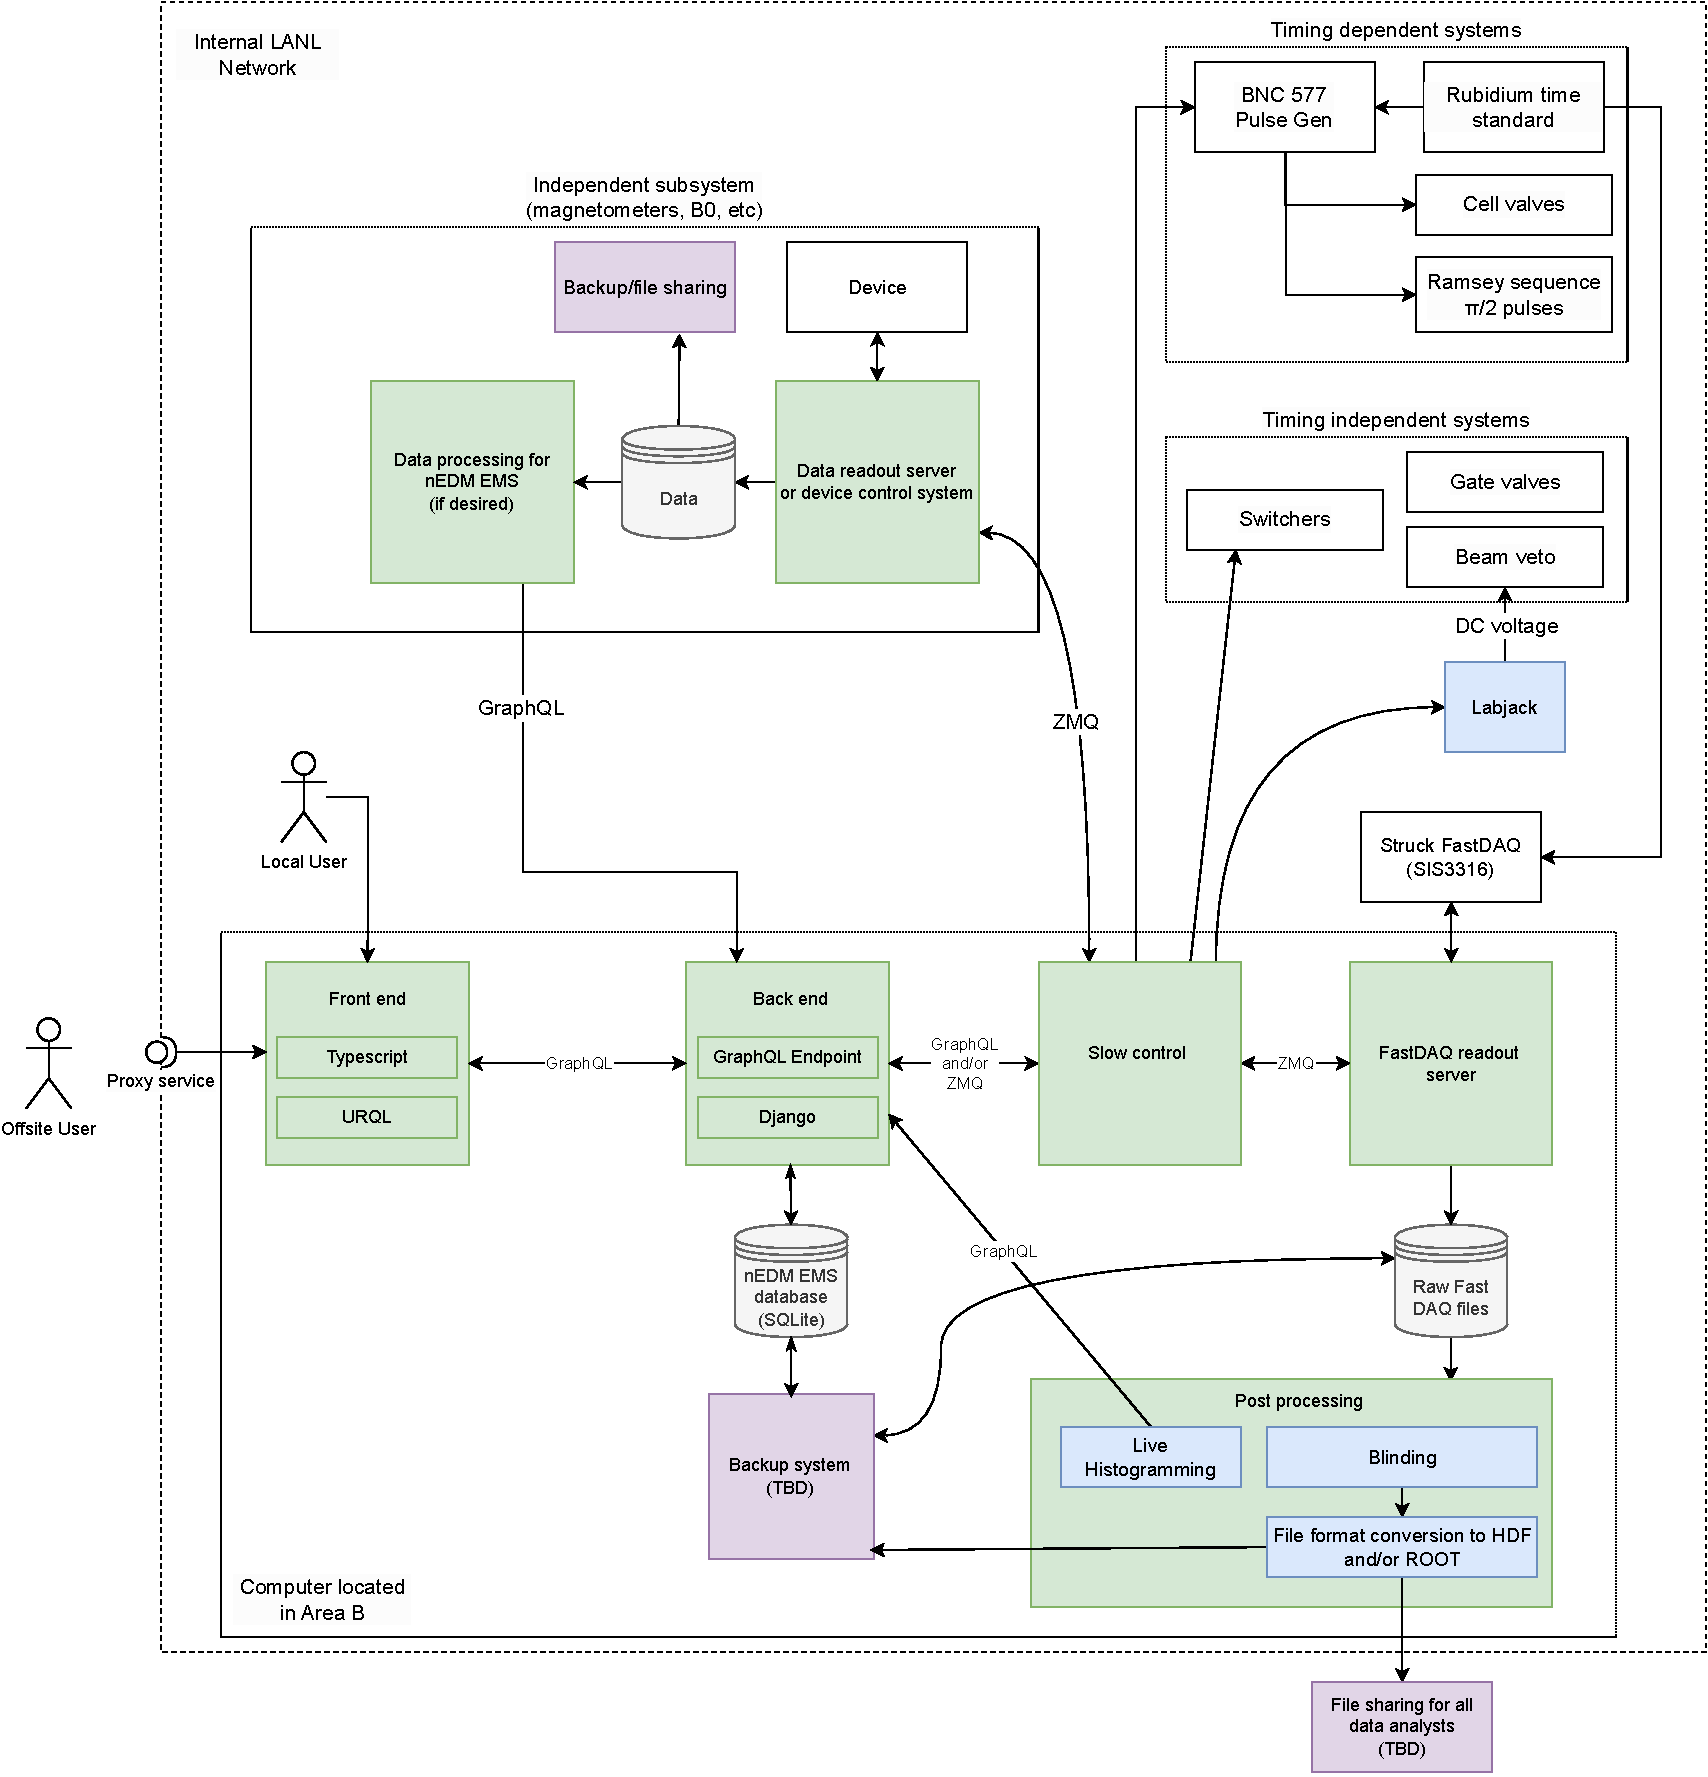
\includegraphics[width=\textwidth]{figures/LANL_nEDM_network.pdf}
    \caption
    [The eventual envisioned experiment control system at LANL]
     {The eventual envisioned experiment control system at LANL, as described in Sec.~\ref{sec:web_control} and demonstrated with a proof of concept [\url{https://github.com/dougUCN/LANE-client}], [\url{https://github.com/dougUCN/LANE-server}]}
    \label{fig:LANL_nEDM_network}
\end{figure}

Again point to git repository

Network map of Frontend to backend

Discuss deployment on LANL network. The domain name system (DNS) is straightforward on the internal LANL network --- a web domain is automatically assigned to each computer. It is then a matter of using Nginx, a reverse proxy, to direct an incoming request to either the front end or backend server. 